\documentclass[fleqn]{IJCAS}  % Comment this line out if you need a4paper
\usepackage{ijcas_packages}

\newcommand{\squeezeup}{\vspace{-2.5mm}}

%%%% Editorial Information
%% Authors do not have to modify this section.
% \journalvolumn{VV}
% \journalnumber{N}
% \journalyear{YYYY}
% \setarticlestartpagenumber{1}
%%%% End of Editorial Information

\newtheorem{definition}{Definition}
\newtheorem{lem}{Lemma}
\newtheorem{prop}{Proposition}
\newtheorem{cor}{Corollary}

\begin{document}

\title{\LARGE \textbf{Awesome title} }

\author{Corresponding Author* and Other authors}%

%%%%%%%%%%%%%%%%%%%%%%%%%%%%%%%%%%%%%%%%%%%%%%%%%%%%%%%%%%%%%%%%%%%%%%%%%%%%%%%%
\begin{abstract}
Great abstract highlighting your hard work
\end{abstract}
%%%%%%%%%%%%%%%%%%%%%%%%%%%%%%%%%%%%%%%%%%%%%%%%%%%%%%%%%%%%%%%%%%%%%%%%%%%%%%%%

\begin{keywords}
attitude control, asymptotic stability, special orthogonal group, constraint
%At least four key words or phrases in alphabetical order, separated by commas.
\end{keywords}

\maketitle % \maketitle command must come here after ABSTRACT and KEYWORDS environments

\makeAuthorInformation{
Manuscript received DATE; revised DATE; accepted DATE.

Authors, Mechanical and Aerospace Engineering, George Washington University, Washington DC 20052 \texttt{ \{EMAIL\}@gwu.edu}

This research has been supported in part by a variety of grants.\\
* Corresponding author.\vskip 0.5pc
}

\runningtitle{1}{Authors}{Running title }


\begin{multicols}{2}
\section{Introduction}\label{sec:intro}

Rigid body attitude control is an important problem for aerospace vehicles, ground and underwater vehicles, as well as robotic systems~\cite{hughes2004,wertz1978}.
One distinctive feature of the attitude dynamics of rigid bodies is that it evolves on a nonlinear manifold.
The three-dimensional special orthogonal group, or \( \SO \), is the set of \( 3 \times 3 \) orthogonal matrices whose determinant is one.
This configuration space is non-Euclidean and yields unique stability properties which are not observable on a linear space.
For example, it is impossible to achieve global attitude stabilization using continuous time-invariant feedback~\cite{bhat2000}.

\section{Problem Formulation}\label{sec:prob_form}
\subsection{Attitude Dynamics}\label{sec:att_dyn}
Consider the attitude dynamics of a rigid body.
We define an inertial reference frame and a body-fixed frame, whose origin is at the center of mass and aligned with the principle directions of the body. 
The configuration manifold of the attitude dynamics is the special orthogonal group:
\begin{align*}
	\SO = \{R\in\R^{3\times 3}\,|\, R^TR=I,\;\mathrm{det}[R]=1\} ,
\end{align*}
where a rotation matrix $R\in\SO$ represents the transformation of the representation of a vector from the body-fixed frame to the inertial reference frame. 
The equations of motion are given by
\begin{gather}
	J\dot\Omega + \Omega\times J\Omega = u+W(R,\Omega)\Delta ,\label{eqn:Wdot}\\
	\dot R = R\hat\Omega ,\label{eqn:Rdot}
\end{gather}
where $J\in\R^{3\times 3}$ is the inertia matrix, and $\Omega\in\R^{3}$ is the angular velocity represented with respect to the body-fixed frame. 
The control moment is denoted by $u\in\R^{3}$, and it is expressed with respect to the body-fixed frame. 
We assume that the external disturbance is expressed by $W(R,\Omega)\Delta$, where $W(R,\Omega):\SO\times\R^{3}\rightarrow \R^{3\times p}$ is a known function of the attitude and the angular velocity.
The disturbance is represented by $\Delta\in\R^{p}$ and is an unknown, but fixed uncertain parameter.
In addition, we assume that a bound on \( W(R, \Omega) \text{ and } \Delta \) is known and given by
\begin{equation}
	\norm{W} \leq B_W , \quad \norm{\Delta} \leq B_\Delta \,, \label{eqn:W_bound}
\end{equation}
for positive constants \( B_W, B_\Delta\).

\begin{prop}[Attitude Error Function] \label{prop:config_error}
%We assume a desired attitude command \( ( R_d, \Omega_d = 0 ) \), the current attitude and angular velocity \( ( R, \Omega) \), and a state constraint~\cref{eqn:constraint} are given.
Define an attitude error function \( \Psi : \SO \to \R \), an attitude error vector \( e_R \in \R^3 \), and an angular velocity error vector \( e_\Omega \in \R^3 \) as follows:
\begin{gather}
	\Psi(R) = A(R) B(R) , \label{eqn:psi} \\
	e_R = e_{R_A} B(R) + A(R) e_{R_B} , \label{eqn:eR} \\
	e_\Omega = \Omega , \label{eqn:eW}
\end{gather}
with
\begin{gather}
	A(R) = \frac{1}{2} \tr{G \left( I - R_d^T R\right)} , \label{eqn:A} \\
	B(R) = 1 - \frac{1}{\alpha} \ln \left( \frac{\cos \theta -  r^T R^T v}{1 + \cos \theta}\right) . \label{eqn:B} \\
	e_{R_A} = \frac{1}{2} \parenth{G R_d^T R - R^T R_d G} ^ \vee , \label{eqn:eRA} \\
	e_{R_B} = \frac{ \left( R^T v\right)^\wedge r}{\alpha \left(r^T R^T v - \cos \theta \right)} . \label{eqn:eRB} 
\end{gather}	
where \( \alpha \in \R \) is defined as a positive constant and the matrix \( G \in \R^{3 \times 3} \) is defined as a diagonal matrix matrix for distinct, positive constants \( g_1, g_2, g_3 \in \R \).
Then, the following properties hold
\begin{enumerate}[(i)]
	\item \label{item:prop_psi_psd} \(\Psi\) is positive definite about \( R = R_d\) on $\SO$.
	\item \label{item:prop_era}The variation of \( A(R) \) with respect to a variation of \( \delta R = R \hat{\eta} \) for \( \eta \in \R^3 \) is given by
	\begin{align}
		\dirDiff{A}{R} &= \eta \cdot e_{R_A} .
	\end{align}
	\item \label{item:prop_erb} The variation of \( B(R) \) with respect to a variation of \( \delta R = R \hat{\eta} \) for \( \eta \in \R^3 \) is given by
	\begin{align}
		\dirDiff{B}{R} &= \eta \cdot e_{R_{B}} .
	\end{align}
%	\item \label{item:prop_crit}The error function \( \Psi \) is minimized when \(R = R_d\).
	\item \label{item:prop_era_upbound}An upper bound of \( \norm{e_{R_A}} \) is given as:
	\begin{align}
		\norm{e_{R_A}}^2 \leq \frac{A(R)}{b_1} , \label{eqn:psi_lower_bound}
	\end{align}
	where the constant \( b_1 \) is given by \( b_1 = \frac{h_1}{h_2 + h_3} \) for 
	\begin{align*}
		h_1 &= \min\braces{g_1 + g_2, g_2 + g_3 , g_3 + g_1} ,\\
		h_2 &= \min\braces{\parenth{g_1 -g_2}^2,\parenth{g_2 -g_3}^2 , \parenth{g_3 -g_1}^2} ,\\
		h_3 &= \min\braces{\parenth{g_1 + g_2}^2, \parenth{g_2 + g_3}^2 , \parenth{g_3 + g_1}^2}.		
	\end{align*}
\end{enumerate}
\end{prop}
\begin{proof}
See~\Cref{proof:config_error}
\end{proof}

\Cref{eqn:psi} is composed of an attractive term, \( A (R) \) toward the desired attitude, and a repulsive term, \( B(R) \) away from the undesired direction \( R^T v \).
In order to visualize the attitude error function on \( \SO \), we utilize a spherical coordinate representation.
Recall, that the spherical coordinate system represents the position of a point relative to an origin in terms of a radial distance, azimuth, and elevation.
This coordinate system is commonly used to define locations on the Earth in terms of a latitude and longitude.
Similarly, the positions of celestial objects are defined on the celestial sphere in terms of right ascension and declination. 
\begin{figure}[H]%
    \centering 
    \subfigure[Attractive \( A(R) \) \label{fig:attract_error}]{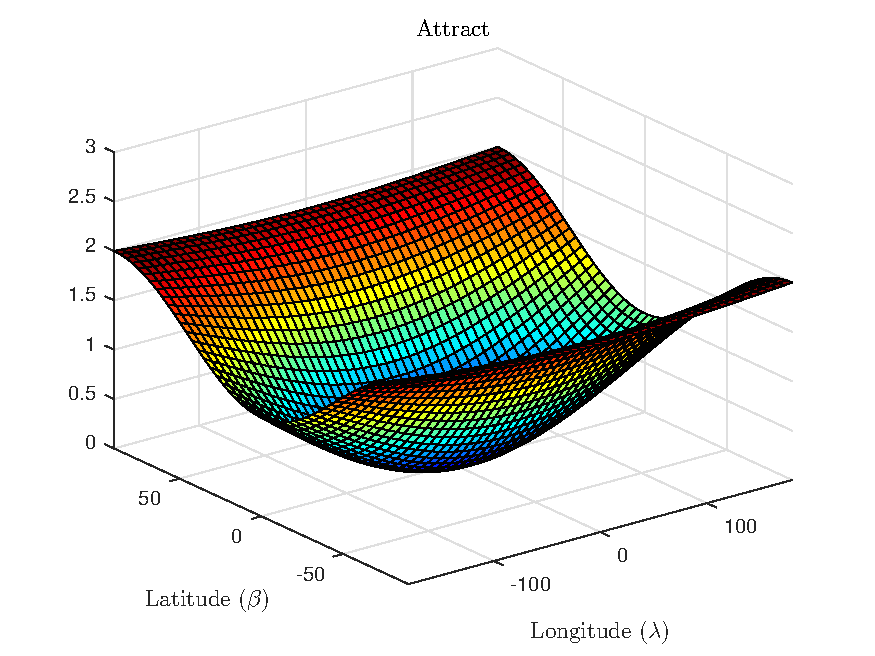
\includegraphics[width=0.45\columnwidth]{attract_error} }~
    \subfigure[Repulsive \( B(R) \) \label{fig:avoid_error} ]{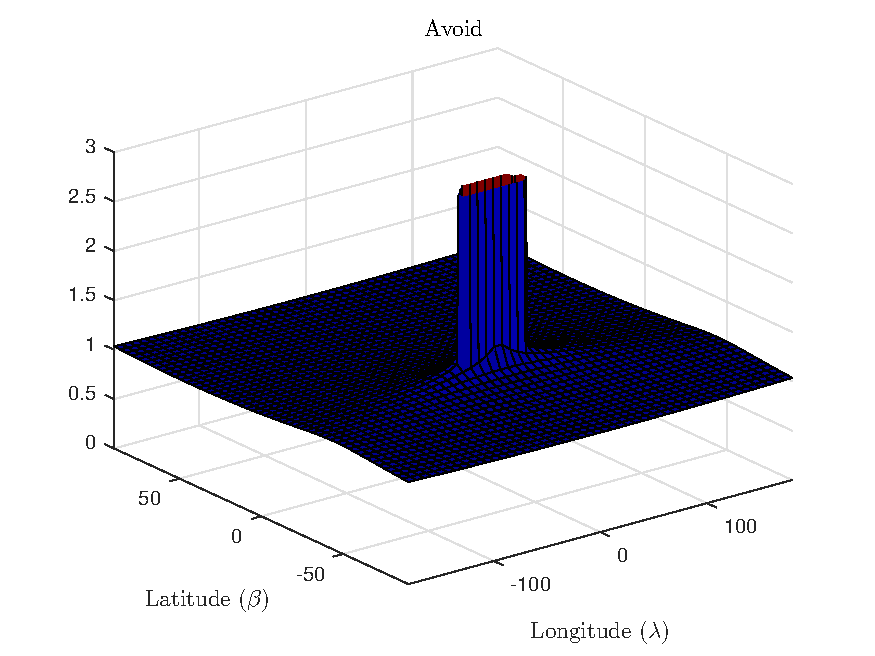
\includegraphics[width=0.45\columnwidth]{avoid_error} }\\%add desired spacing between images, e. g. ~, \quad, \qquad, \hfill etc. %(or a blank line to force the subfigure onto a new line) 
    \subfigure[Configuration \( \Psi \) \label{fig:combined_error}]{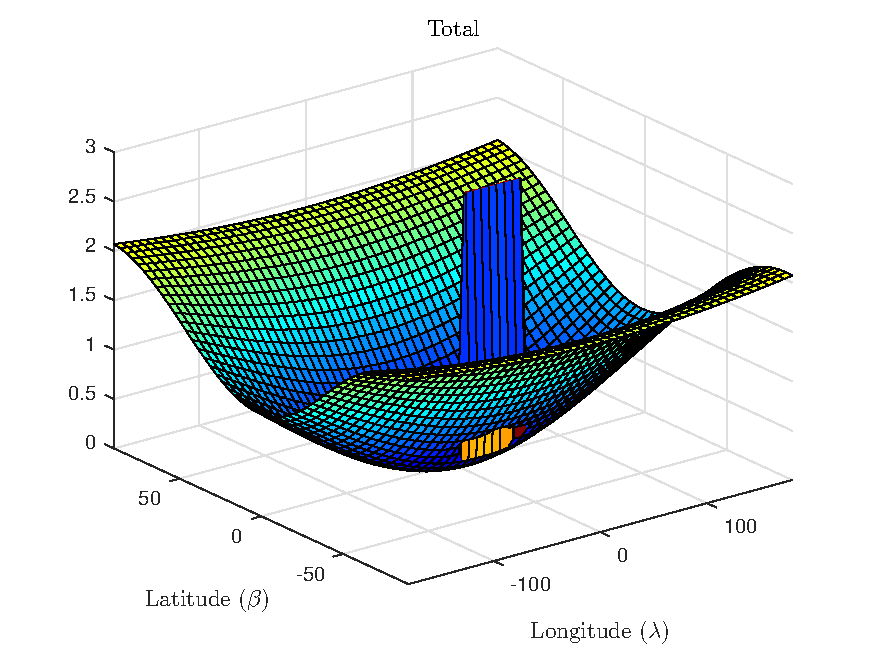
\includegraphics[width=0.45\columnwidth]{combined_error} }%
    \caption{Configuration error function visualization}
    \label{fig:config_error} 
\end{figure}%

\subsection{Attitude Control without Disturbance}

\subsection{Adaptive Control}



\section{Conclusions}\label{sec:conclusions}
Awesome conclusion

%%%%%%%%%%%%%%%%%%%%%%%%%%%%%%%%%%%%%%%%%%%%%%%%%%%%%%%%%%%%%%%%%%%%%%%%%%%%%%%%
\appendix
\subsection{Proof of~\Cref{prop:config_error}}\label{proof:config_error}
To prove~\cref{item:prop_psi_psd}, we note that~\cref{eqn:A} is a positive definite function about \( R = R_d \)~\cite{bullo2004}.
The constraint angle is assumed \( \ang{0} \leq \theta \leq \ang{90} \) such that \( 0 \leq \cos \theta \).
The term \( r^T R^T v \) represents the cosine of the angle between the body fixed vector \( r \) and the inertial vector \( v \). 
It follows that
\begin{align*}
	0 \leq  \frac{\cos \theta -  r^T R^T v}{1 + \cos \theta} \leq 1 ,
\end{align*}
for all \( R \in \SO \). 
As a result, its negative logarithm is always positive and from~\cref{eqn:B}, \(1 < B\).
The error function \( \Psi = A B \) is composed of two positive terms and is therefore also positive definite.

%\addtolength{\textheight}{-12cm}   % This command serves to balance the column lengths
                                  % on the last page of the document manually. It shortens
                                  % the textheight of the last page by a suitable amount.
                                  % This command does not take effect until the next page
                                  % so it should come on the page before the last. Make
                                  % sure that you do not shorten the textheight too much.
                                  
\bibliography{BibMaster,library}
\bibliographystyle{IEEEtran}

\biography{profile}{Shankar Kulumani}
    {is a PhD Candidate in the Department of Mechanical and Aerospace Engineering at George Washington University. 
    He received his bachelor's degree in Astronautical Engineering from the United States Air Force Academy in 2009 and his master's in Aeronautical and Astronautical Engineering from Purdue University in 2013.
    % He previously served as Deputy Space Vehicles Lead for the ORS-1 (Operationally Responsive Space ) satellite program, and as Lead Test Engineer in the Guidance, Navigation, and Control group at Air Force Research Laboratory located at Kirtland AFB, NM.
    % He is now currently a reserve air force officer where he serves as Threat Systems Engineer for the Missle and Space Intelligence Center, Defense Intelligence Agency.
    His current research interests include the application of geometric mechanics and control to aerospace systems. 
    }

\biography{Lee}{Taeyoung Lee}
    {is an associate professor of Department of Mechanical and Aerospace Engineering at the George Washington University. 
    He received his doctoral degree in Aerospace Engineering and his master's degree in Mathematics at the University of Michigan in 2008. 
    His research interests include computational geometric mechanics and control of complex systems.}    
\clearafterbiography\relax
\clearafterbiography\relax
\end{multicols}

\end{document}
